% PLEASE USE THIS FILE AS A TEMPLATE
% Check file iosart2x.tex for more examples

% add. options: [seceqn,secthm,crcready]
\documentclass[sw]{iosart2x}
\usepackage{todonotes}
\usepackage{cleveref}
\usepackage{csquotes}
\usepackage{aurl}
\usepackage{booktabs}
%\usepackage{dcolumn}

%%%%%%%%%%% Put your definitions here
\newcommand{\aw}{AnthroWorks3D}
\daurl{anno}{https://annosaxfdm.de/ontology/}

%%%%%%%%%%% End of definitions

\pubyear{2023}
\volume{0}
\firstpage{1}
\lastpage{1}

\begin{document}

\begin{frontmatter}

%\pretitle{}
\title{The Anthropological Notation Ontology (ANNO): A core ontology for annotating human bones and deriving phenotypes}
\runtitle{Anthropological Notation Ontology}
%\subtitle{}

% For one author:
%\author{\inits{N.}\fnms{Name1} \snm{Surname1}\ead[label=e1]{first@somewhere.com}}
%\address{Department first, \orgname{University or Company name},
%Abbreviate US states, \cny{Country}\printead[presep={\\}]{e1}}
% Höffner, Heuschkel, Schmiedel, Penne, Fritzsch, Ludwig, Mohaupt, Labudde, Uciteli
% TODO: overleaf
% Two or more authors:
\begin{aug}
\author[B]{\inits{M.}\fnms{Marie} \snm{Heuschkel}\ead[label=e2]{marie.heuschkel@hs-mittweida.de}}
\author[A]{\inits{K.}\fnms{Konrad} \snm{Höffner}\ead[label=e1]{konrad.hoeffner@uni-leipzig.de}%
\thanks{Corresponding author. \printead{e1}.}
\thanks{Equal contribution.}%how to show this for the first 3?
}
\author[B]{\inits{F.}\fnms{Fabian} \snm{Schmiedel}\ead[label=e3]{fabian.schmiedel@hs-mittweida.de}}
\author[B]{\inits{L.}\fnms{Laura} \snm{Penne}\ead[label=e4]{laura.penne@hs-mittweida.de}}
\author[B]{\inits{H. T.}\fnms{Hanjo Tim} \snm{Fritzsch}\ead[label=e5]{fritzsc2@hs-mittweida.de}}
\author[B]{\inits{N.}\fnms{Niklas} \snm{de Sousa Norte}\ead[label=e6]{niklas.desousanorte@hs-mittweida.de}}
\author[B]{\inits{A.}\fnms{Andrea} \snm{Ferencová}\ead[label=e7]{andrea.ferencova@hs-mittweida.de}}
\author[B]{\inits{A.}\fnms{Andy} \snm{Ludwig}\ead[label=e8]{andy.ludwig@hs-mittweida.de}}% ist jetzt beim Fraunhofer, möchte aber weiter so gelistet werden
\author[B]{\inits{M.}\fnms{Marleen} \snm{Mohaupt}\ead[label=e9]{kreuzer@hs-mittweida.de}}
\author[B]{\inits{D.}\fnms{Dirk} \snm{Labudde}\ead[label=e10]{dirk.labudde@hs-mittweida.de }}
\author[A]{\inits{A.}\fnms{Alexandr} \snm{Uciteli}\ead[label=e11]{alexander.uciteli@imise.uni-leipzig.de}}
%\author[B]{\inits{}\fnms{} \snm{}\ead[label=e9]{}}
\address[A]{Institute for Medical Informatics, Statistics and Epidemiology (IMISE), \orgname{Leipzig University},
Saxony, \cny{Germany}\printead[presep={\\}]{e1,e11}}
\address[B]{\orgname{Hochschule Mittweida},
Saxony, \cny{Germany}\printead[presep={\\}]{e2,e3,e4,e5,e6,e7,e8,e9,e10}}
\end{aug}

%\begin{review}{editor}
%\reviewer{\fnms{First} \snm{Editor}\address{\orgname{University or Company name}, \cny{Country}}}
%\reviewer{\fnms{Second} \snm{Editor}\address{\orgname{First University or Company name}, \cny{Country}
%  and \orgname{Second University or Company name}, \cny{Country}}}
%\end{review}
%\begin{review}{solicited}
%\reviewer{\fnms{First} \snm{Solicited reviewer}\address{\orgname{University or Company name}, \cny{Country}}}
%\reviewer{\snm{anonymous reviewer}}
%\end{review}
%\begin{review}{open}
%\reviewer{\fnms{First} \snm{Open Reviewer}\address{\orgname{University or Company name}, \cny{Country}}}
%\end{review}

\begin{abstract}
The Anthropological Notation Ontology (ANNO) allows the systematic, standardised classification of recovered bone finds into the skeletal system, the description of the skeletal pieces, and the definition of functions for the derivation of different phenotypes of humans in forensic and historical anthropology.
ANNO consists of two components:
ANNOdc, a domain-core ontology providing core entities such as basic anatomical categories, and ANNOds, a domain-specific ontology used for annotating structures of the human skeleton.
ANNO is integrated into AnthroWorks3D (AW3D), an application for the creation and analysis of 3D-models of human skeletal remains.
The integration is based on the three-ontology method with the General Formal Ontology as the top level ontology, ANNOdc as the task ontology and ANNOds as the domain ontology.
Thus, AnthroWorks3D only needs to implement access to the entities (classes and properties) of the task ontology, whereas the entities of the corresponding domain ontology are processed dynamically.
ANNO supports the analysis of skeletal and bone finds in forensic and historical anthropology, facilitating the standardisation of data annotation and ensuring accurate preservation of information for posterity.
\end{abstract}

\begin{keyword}
\kwd{Ontology}
\kwd{Ontology development}
\kwd{Anthropology}
\end{keyword}

\end{frontmatter}

%%%%%%%%%%% The article body starts:
% TODO notes from meeting, einarbeiten:
% 3 Teile Kernmodule mit Use Cases, weitere Komponenten durch Community


\section{Introduction}\label{sec:introduction}

Data from historical and prehistoric anthropology~\citep{prehistoricanthropology}, as well as modern forensic science, allows for a comprehensive understanding of deceased individuals from different time periods, ranging from their identity and health status to aspects of their behaviour, lifestyle, culture and even concerning the circumstances of their death~\citep{spurensuche}.
For example, anthropological methods can be used to determine individual properties (phenotypes) such as their sex, age, height and ancestry and further individualising traits.

Digitalisation offers several advantages to anthropology, including remote work, without the effects of wear and tear on the physical skeletal specimens.
Current problems of access can be resolved, as examinations can be conducted even if the skeletal material from individuals or collectives are not present at the institution or may have already been reburied, which facilitates interdisciplinary collaborative research.
Moreover it allows for linking data of different study samples across geographical boundaries.
Data sets consolidated this way and formalised through the Anthropological Notation Ontology (ANNO) presented here allow for efficient data analysis techniques, such as data and text mining that promote deeper insights.

Apart from contextual information, most informative clues can be found directly on the bone.
Anthropologists use human anatomy, specifically the skeletal system and further tissues of the musculoskeletal system, to classify and describe and thus document bones, anatomical structures and diagnostic features within the overall framework of the skeleton in a comprehensive and transparent fashion.

Applying the same principles used for mapping the Earth’s surface \enquote{terrain}, it is possible to create a detailed map of the human body containing visible anatomical surface structures as well as artificial objects such as measurement points or content-related or methodologically based classifications and boundaries~\citep{topo}. ANNO represents such a map by providing an ontology for accurate and exhaustive definitions that allow to unequivocally locate these, ensure their easy retrieval and furthermore serve as a basis for the objective examination, for instance in the form of measurements.


ANNO consists of two components: ANNOdc, a domain-core ontology providing core entities such as basic anatomical concepts and classifications, and ANNOds, a domain-specific ontology employed for annotating human skeletal structures. In its current version, the ontology  refers to standardised normal adult anatomy, excluding developmental aspects, variations, pathologies and other related factors. ANNO is integrated into AnthroWorks3D (AW3D), an application for generating and analysing 3D-models of human skeletal remains. 


\section{Related Work}

There are various reference materials for the description of anatomical structures, ranging from anatomical atlases to nomenclatures.
The latter aim for an established standardised naming and systematisation.
There are currently two prominent ontologies in the field of general anatomy:

The Terminologia anatomica~\citep{ta2} (TA) is a hierarchy of anatomical structure concepts for the entire human body.
For historical reasons, it uses a terminology consisting of Latin and originally Greek, which was later latinised.
For each anatomical structure, the TA provides the \enquote{preferred}, i.e. standard, Latin term and its English equivalent as well as an individual identification number.
In some cases, Latin and English synonyms are also included, e.g. \emph{malar bone} is an English synonym of the Latin preferred term \emph{Os zygomaticum} and its English equivalent \emph{zygomatic bone}.
The identification number is crucial, as certain landmarks are mostly listed without bone affiliation, resulting in multiple occurrences. %(s. Bone Part)
For instance, the \emph{processus zygomaticus} can be found both at the \emph{os frontale} and the \emph{os temporale}.
Eponyms are terms derived from proper nouns such as the name of a person, place or thing, and they are considered a type of synonyms since they stand for the same anatomical structure.
For example, \emph{ossa digitorum manus / pedis} (engl. \emph{phalanges of the hand / foot}) are the small bones of the fingers and toes and are also denoted as \emph{phalanges manus / pedis} which are named after the Greek word \emph{phalanx} for a dense rectangular infantry formation.
In addition to the outdated print edition~\citep{ta1998}, an extended second edition (TA2) is available online~\citep{ta2}.
Furthermore, there is a commercially available independent companion print publication with German~\citep{anatomylexicon}, English~\citep{pocketatlas} and Spanish~\citep{taspanish} editions of which at least the German edition is regularly updated.
This book contains textual and visual descriptions, whereby anatomical structures are indicated through lines on the illustrations.

The \emph{Foundational Model of Anatomy} (FMA)~\citep{fma} ontology represents the physical organisation of human anatomy by mapping relations to one another.
It allows the knowledge it contains to be represented in a way that is humanly comprehensible and machine-interpretable.
The FMA uses the Basic Formal Ontology (BFO) as its top level ontology.
Corresponding to its relational nature, new higher level concepts are introduced and used for reorganising the actual anatomical structures diverging from the TA’s hierarchical structure.
Thus, in 90\,\% of the cases this lead to new creations of anatomical concepts~\citep{anatomicalterms} whereas only 1\,\% contain textual definitions~\citep{uberon}.

We manually created links to FMA.
Wikidata provides unofficial links between the FMA and TA2 which we use to link to TA2.

\subsection{Problems and Research Gaps}

There are several issues and research gaps when it comes to naming and defining anatomical concepts and instances that neither current ontologies nor reference literature---general or subject-specific---can address adequately so far.

The primary issue lies in the absence of standardisation.
While both the TA and FMA have been proposed as a means of standardising terminology, they haven't garnered sufficient acceptance to facilitate the adoption of a unified and consistent body of work to establish standardisation in actual practice~\citep{frequencyta,doestamatter,athighlights}.
Instead, the usage of terminology is as fluent as any other language, depending on its socio-cultural environment, such as schools or language areas~\citep{doestamatter,atthennow,atinfo,frequencyta,atcompare}.
Thus, the usage of English designations is preferred in the Anglo-American sphere while Latin terms are commonly used in German-speaking areas~\citep{anatomycontribution,anatomylexicon,reforminganatomical}.
As a consequence there are at times various translations for the same anatomical terms~\citep{naminggame}.
Yet, knowledge of Latin is generally declining.
With the terms hence becoming more abstract to the people using them, there is also a common prevalence for spelling divergences or grammar mistakes~\citep{ta17,anatomylexicon,athighlights,diphthongs}.
Moreover, in textual descriptions latin and the native language are commonly used interchangeably for stylistic purposes.
For instance, \cite{anatomylexicon} uses the German terms of the bones in the explanation of sutures.
Meanwhile, the existing terminology is not flexible enough for language-like usage as, for example, there is an inconsistent use of singular and plural forms or gaps in lateralized landmarks.

If not historically evolved, anatomical terms usually correspond to a description of the location, affiliation or function of the respective concept or structure~\citep{reforminganatomical}.
However, this kind of naming variable, non-intuitive and therefore inconsistent.
An example, showing the variability in illustrative descriptions are the Tuberculum articulare of the Processus zygomaticus, which in \cite{anatomie} is described as saddle-shaped although it is not called \emph{sella}, the Latin name for saddle.
It is moreover worth pointing out that not every anatomical structures contributing to an articulation in some way, automatically carry the term articular with them, such as the Caput mandibulae, which connects the Mandibula to the rest of the Cranium.
The Tuber frontale, which serves as an indicator for sex in anthropology, is listed as an eminentia in the TA~\citep{ta2}.
Likewise, he Protuberantia mentale is referred to as Eminentia mentale in a widely-used anthropological method that is also used for sex determination.
As can be seen, the incentive for synonyms is high.
However, the current resources fail to provide comprehensive lists of synonyms in use.
 This in turn may lead to misattribution, as is the case for example, in the FMA the entry with the \emph{preferred name} \enquote{External acoustic aperture} and \emph{non-English equivalent} \enquote{Porus acusticus externus} (FMA ID: 61301) lists external acoustic meatus (Meatus acusticus externus in Latin) as a synonym.
However, it is not the same, rather the Porus is---as its English name indicates---the opening to the meatus~\citep{anatomylexicon}.
%Furthermore, terms oftentimes lack clear affiliation to the bone to which they belong.
%When considering the whole skeleton, these terms consequently occur multiple times, causing ambiguity.
Occasionally, there are discrepancies and inconsistencies found in the definitions of individual anatomical structures.
For instance, the position of the Corpus ossis pubis varies across different sources~\citep{anatomylexicon,prometheus,allgemeineanatomie,dualereiheanatomie,anatomiedesmenschen}.

%In addition, the ontologies are only inadequately (TA for the last time in 2013, FMA in 2020) updated and do not undergo continuous synchronisation.%add source for that? 11 and 12 in table but no paper.
Another main issue is that neither FMA nor TA are tailored to fit the requirements of anthropology or any other specialised field~\citep{fma}.
For example, articular surfaces of the individual bones are relevant anthropologically, yet not all articular surfaces (e.g. on the Ossa carpi or Ossa metatarsi) are defined in the TA or FMA, resulting in further gaps.
A similar situation exists with respect to osteometric measurements.
Established and to some extent standardised osteometric measurement points are only found on the cranium and mandible~\citep{wesenanthropologie}.
 However, since there are measurement distances on all bones, the respective start and end points must also be defined.
Last but not least, both ontologies suffer from a lack of consideration given to anatomical variants~\citep{anatomycontribution}.
Moreover, different disciplines require a different level of detail, which is why nose surgery works with anatomical terms of very detailed anatomical structures~\citep{graysanatomy},
which to the greater part are not found in the FMA or the TA that primarily aim for the standardisation of general (clinical) anatomy~\citep{fma}.
A work of dental anthropology even split the aforementioned Tuberculum articulare (Articular tubercle) in two structures, naming the other \enquote{articular eminence}~\citep{dentalanthropology}.
%Often exchange between these specific fields and general anatomy hardly takes place.
It stands to reason that interdisciplinary coordination between the individual disciplines and general anatomy hardly takes place.

Furthermore, visual representation of anatomical structures is frequently missing or insufficient in anatomical resources.
The labelling is often selective, varies by source and is mostly limited to arrows as a means for local designation.
However, since they are multi-dimensional structures, it is essential to provide a marker over the entire landmark and delineate it accurately.
The latter also requires a clear textual definition.
 However, there are currently no equivalent standardised definitions for skeletal anatomy, meanwhile anatomical resources only provide sparse information on the topic.

For these reasons, it is necessary to develop unified, textual, visual, and detailed descriptive definitions for anatomical concepts and instances.
Additionally, these should be presented in a clear way within an ontology that is easy to understand by the user.

%\url{https://bioportal.bioontology.org/ontologies/FMA}

\section{Ontological Architecture}\label{sec:architecture}

The ontological architecture of ANNO consists of three interrelated layers representing by a top-level ontology, a domain-core ontology and a domain-specific ontology:

\begin{enumerate}
\item We use the General Formal Ontology (GFO)~\citep{gfo} as top-level ontology of ANNO.
In the current paper, we refer especially to the categories \enquote{Material object}, \enquote{Attributive}, \enquote{Relator} as well as the spatial entities of GFO (\cref{sec:core}, \cref{fig:gfo})

\item ANNOdc (\cref{sec:core}, \cref{fig:core}) is a domain-core (dc) ontology to provide the core entities of a domain.
This includes general anatomical categories (Bone and Tooth), a category for describing their characteristics (Anatomical property), anatomical spatial entities (Anatomical space, surface, line and point) as well as the category \emph{Phenotype} to model the rules for determining human phenotypes.
ANNOdc is embedded in the GFO, i.e. the ANNOdc classes are subclasses of GFO classes.

\item ANNOds (\cref{sec:domain}) is a domain-specific (ds) ontology for describing domain-specific entities to be used for annotating the parts of the human skeleton.
These are bones, teeth, their parts and compounds, such as \emph{mandible}, \emph{Mental protuberance} or the facial skeleton.
It is also used for modelling their properties and relations, such as the distance between Mentale dexterum and Mentale sinistrum, needed to derive human phenotypes like sex or height.
ANNOds is embedded in ANNOdc.
\end{enumerate}

% take care to prevent the problems noted by reviewer 1 in https://semantic-web-journal.net/content/modelling-digital-health-data-examode-ontology-histopathology
% TODO: ontology language, expressivity
% TODO: reuse of ontological entities
% TODO: clear validation mechanism
% TODO: top-level ontology?

\section{Description and Foundation of ANNOdc}\label{sec:core}
% Definition/Beschreibung der Kern-Konzepte/Module und -Relationen mit Beispielen, GFO-Einbettung
\begin{figure}[h]
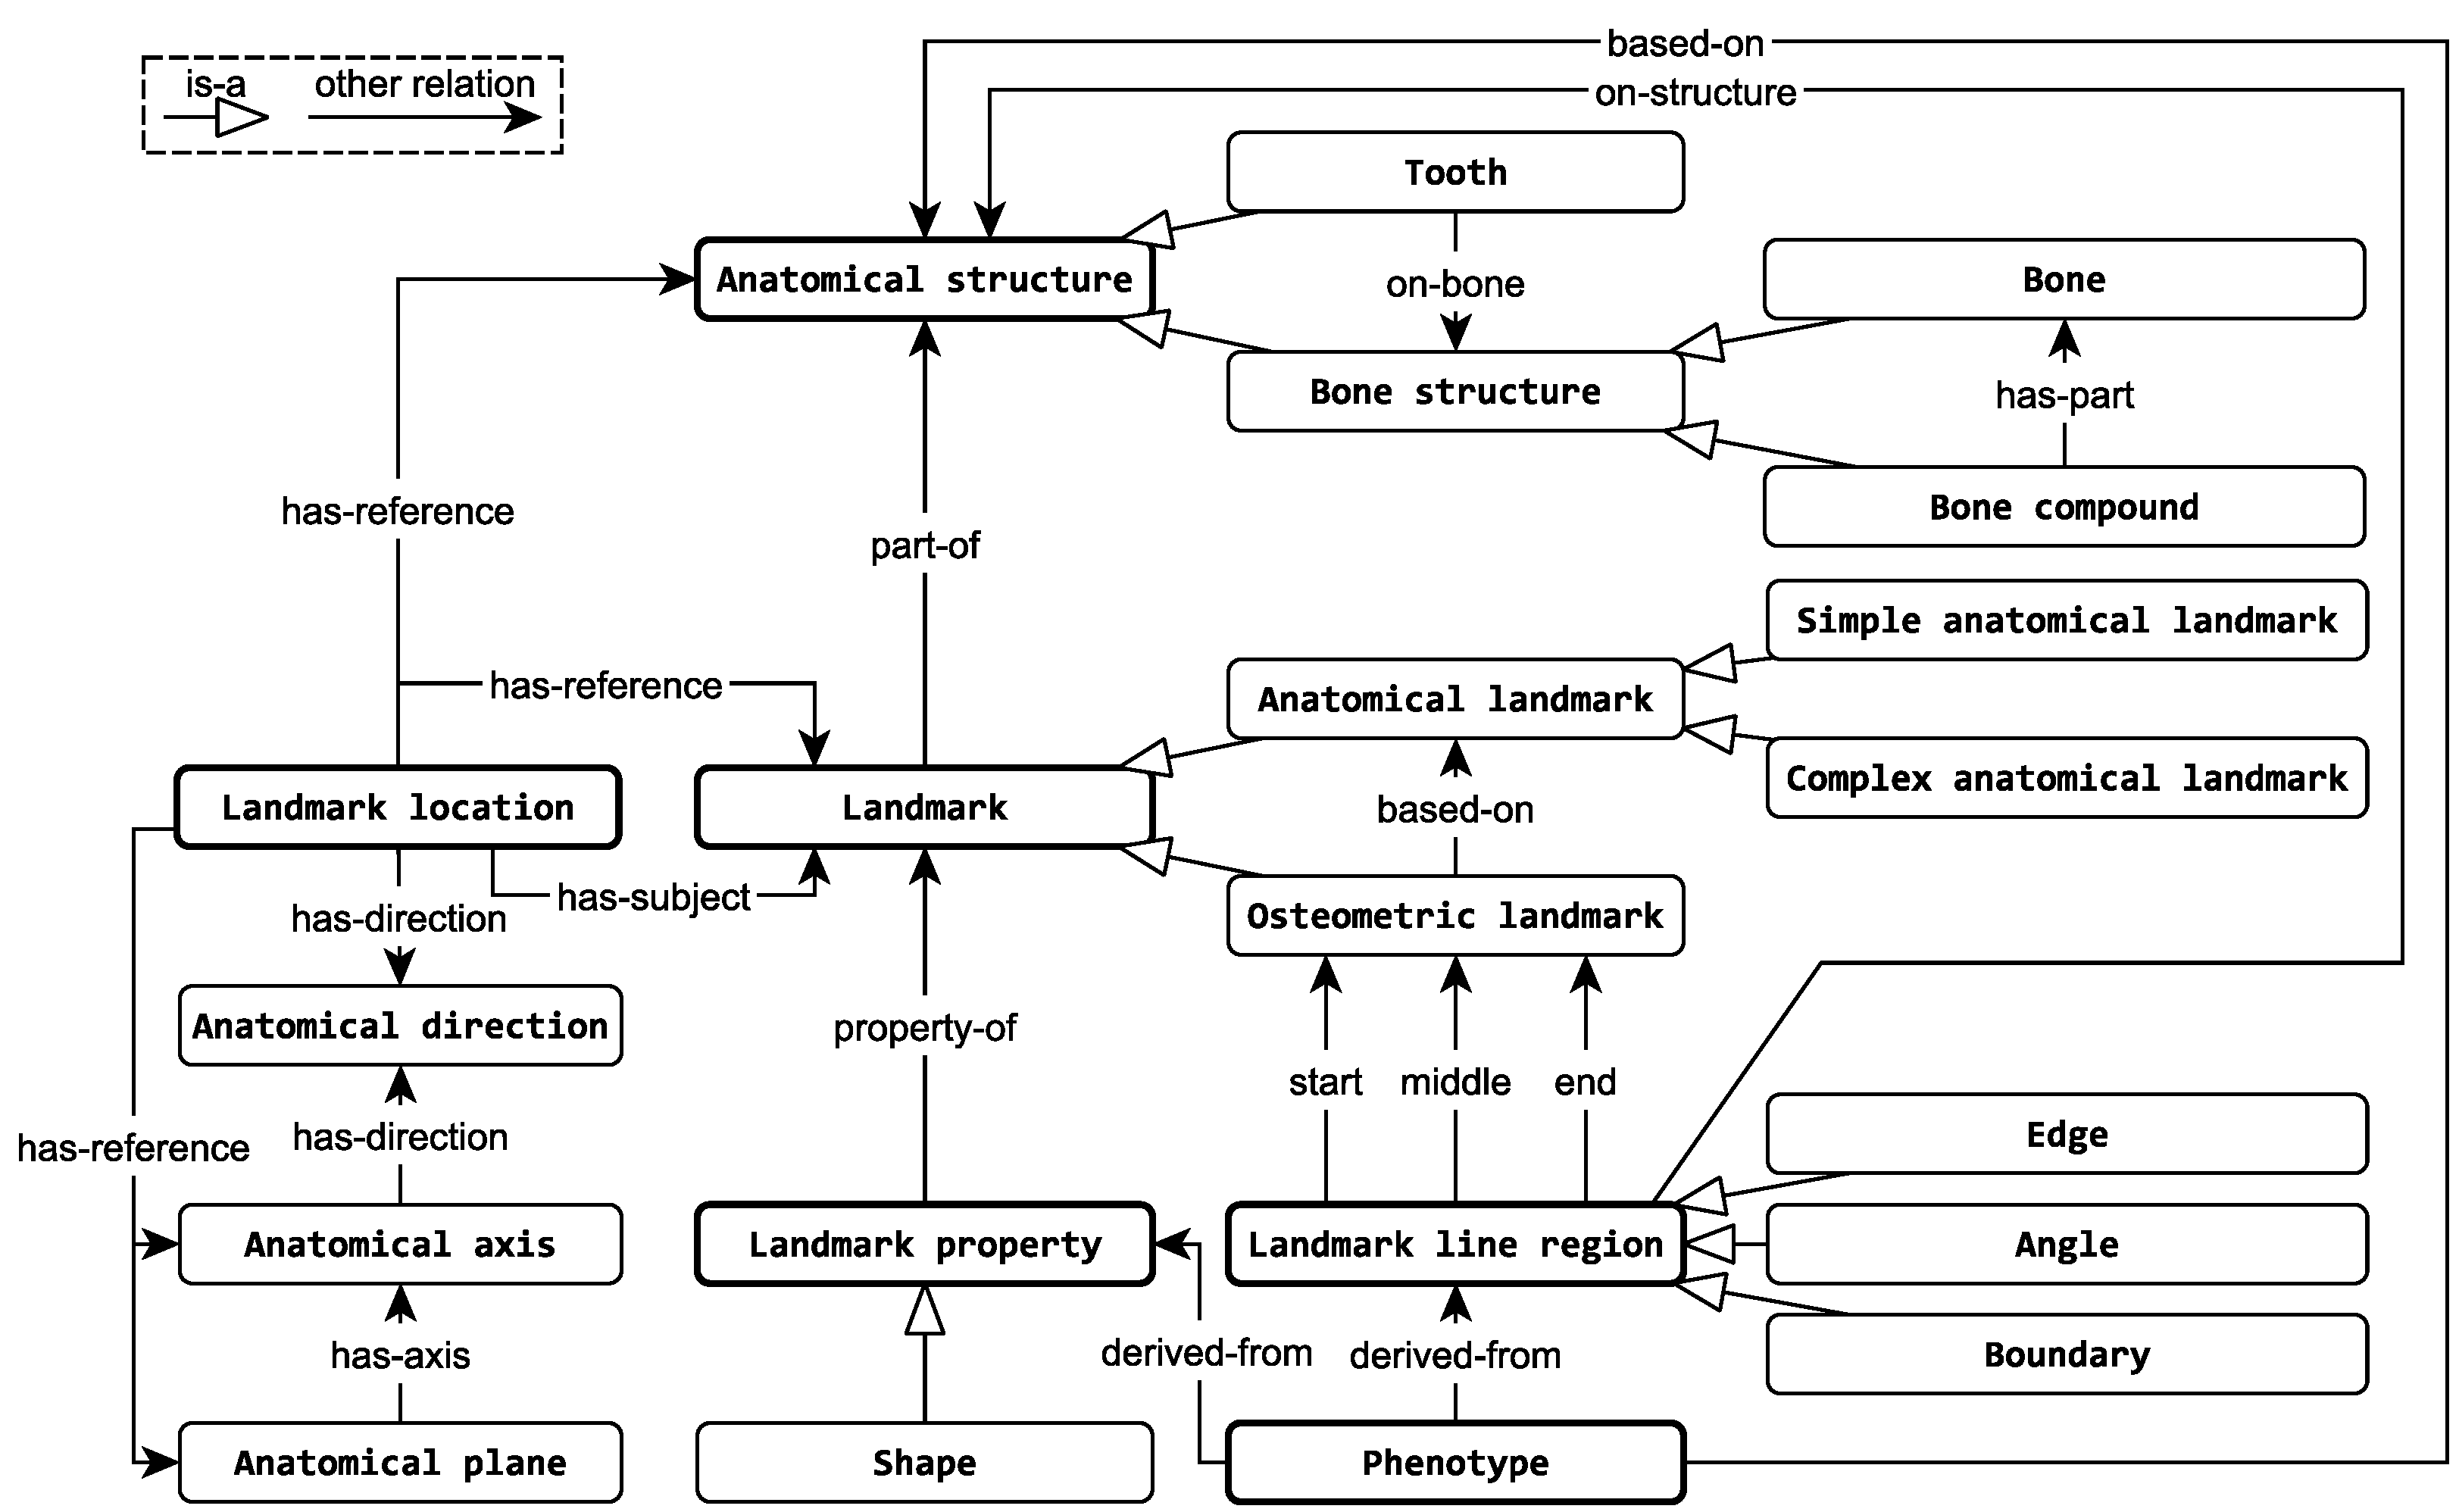
\includegraphics[width=\textwidth]{img/core.pdf}
\caption{ANNOdc ontology}\label{fig:core}
\end{figure}

\begin{table}[htbp]
  \centering
  \caption{Table Title}
  \begin{tabular}{llll}
    \toprule
	ANNOdc class					&Examples				&FMA equivalent / ID						&GFO superclass	\\
	\midrule
	Anatomical entity				&						&Physical anatomical entity fma61775\\
	Anatomical structure			&						&Material anatomical entity	fma67165		&Material object\\							
	Spatial anatomical entity		&						&immaterial anatomical entity fma:fma67112	&Space entity\\
	Anatomical space				&						&											&Space region\\
	Anatomical surface				&Median Plane			&Anatomical surface fma24137				&Surface region\\
	Anatomical line					&Mandibular Angle (ppam dexter-go dexter-piam dexter), Sagittal Axis	&Anatomical line fma9657	&Line region\\
	Anatomical point				&Gonion					&Anatomical point							&Point region\\
	Anatomical plane				&Median Plane			&Anatomical plane fma242982\\
	Anatomical axis		 			&Sagittal Axis\\
	Skeleton						&						&Skeleton fma:fma23875\\
	Bone structure\\
	Bone							&Mandibula			&Bone organ fma:fma5018					&-				\\
	Bone part					&-					&Protuberantia mentalis					&Related to Segment of bone organ fma:fma281808, Zone of bone organ fma:fma10483\\
	Bone compound				&Cranium				&Comparable to union of Skeletal system fma:fma23881 and subdivision of skeletal system fma:fma85544&-\\
	Tooth structure				&Dentes Permanentes	&Permanent teeth (fma:fma75152; TA2ID:913)&Tooth			\\
	Tooth						&Dens caninus			&Tooth fma:fma12516						&-				\\
	Tooth part					&Cuspis dentis		&fma:fma56481; TA2ID:925					&-				\\
	Phenotype					&Height, Sex			&-										&Anatomical Property\\
	Attributive					&Anatomical relation, e.g., Has\_shape relation&-							&Attributive	\\
	Anatomical qualitative coordinate&Superior, lateral, medial, posterior&Anatomical Property	&Relator		\\
\bottomrule
\end{tabular}
\end{table}


\begin{figure}[h]
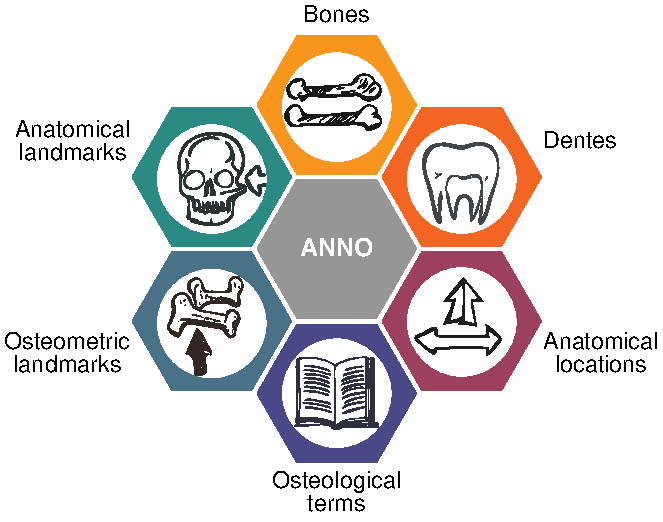
\includegraphics[width=0.3\textwidth]{img/modules.pdf}
\caption{The six modules of ANNO}\label{fig:modules}
\end{figure}
\todo{Brauchen wir \cref{fig:modules} noch oder ist sie durch \cref{fig:core} nicht mehr nötig?}

The ontology consists of the following core modules, see \cref{fig:modules}:
%For the categories, there were the following spreadsheets: bones, anatomical landmarks, osteometric landmarks, measured distances, function (separately for discriminant and regress functions), anatomical position descriptions, sources used, and osteological terminology.
\subsection{Anatomical Structures}\label{sec:bone}

In ANNO, we consider bone structures and teeth as anatomical structures relevant to the anthropology domain.
Bone structures are divided into single bones and bone compounds consisting of further bones (has\_part).
Teeth are located on bone structures (on\_bone).

\subsection{Landmarks}\label{sec:landmark}
All landmarks are annotated with their name in singular and plural form, reference bone, synonyms, textual and visual definition, FMA and TA ID, and sources.


\paragraph{Anatomical Landmarks}
Anatomical landmarks are defined either on a bone or an anatomical compound structure.
Landmarks have properties such as shape and phenotypes are derived from those properties.

\paragraph{Osteometric Landmarks}

\subsection{Landmark Properties}

\subsection{Relative Landmark Positions}

A relative position of a landmark regarding a reference object can be described using the ANNO.
For this, the corresponding landmark (the subject), a reference object
(anatomical structure, anatomical axis, anatomical plane or another landmark) and, if required, an anatomical direction
(in relation to the reference object) must be specified. If the direction was not specified, the landmark is located on the reference object.

\subsection{Landmark Line Regions and Measurements}
Landmark line regions are lines connecting or outlining landmarks (e.g., an edge between two landmarks, an angle between three landmarks
or an outline of one or more landmarks). A landmark line region can start on one landmark and end on another,
passing through or bordering multiple landmarks.
The landmark line regions can be measured (e.g., the length of the edge or outline and the angle degree).
Such measurements can be used to derive/determine individual phenotypes.

Measurements consist of references to sections, the start point, midpoint, end point, and short definitions.

\todo{Umschreiben von Modulen auf ANNOdc}
\subsection{Phenotypes and Functions}
Functions are categorized into sex determination and regress functions for body height estimation.
RDF is not optimized for mathematical formulas so we model those as literals.

\paragraph{Sex determination}
% auto translated from the project report, use as basis:
The sex of a specific individual within a population may be estimated using a function on skelettal measurements that is specific to this population.
Based on a threshold value, skeletons are classified into male, probably male, indifferent, probably female, and female.

\paragraph{Regress functions}
Regress functions for body height and body weight estimation.
The goal here was to cover functions for at least one European, African, American, and Asian ethnic group or population.
Names were assigned by the number included in each study, the authors, and the year of publication.
In addition, the function, reference population, aspect (e.g., discriminant function), and sample size with division by gender were noted.
In addition, for the discriminant functions, the thresholds of sex assignment, classification accuracy, and misclassification were important; for the regression functions, the error interval was important.


\subsection{Foundation of ANNO with GFO}

Anatomical structures and landmarks (as parts of anatomical structures) are material objects in the sense of the GFO because they consist of matter, have a mass and occupy space~\citep{gfospace}.
The landmark properties (such as shape) are interpreted as attributives (or qualities) in GFO~\citep{gfoarchitecture}.
These are dependent individuals that characterise other individuals (in our case, the landmarks).
The phenotype notion has already been analysed in detail within the framework of the Core Ontology of Phenotypes and defined as an individual property of an organism (such as sex or body height)~\citep{ontologicalrepresentation}.
The phenotypes are therefore also attributives in the GFO sense.
The relative position (location) of a landmark with respect to another entity is represented by GFO relators.
Relators are instances of relations, are composed of roles and link other entities together~\citep{gfocategory}.
The landmark location relator consists of three roles: subject (the landmark whose position should be described), the reference object (anatomical structure, landmark, axis or plane) and the direction (e.g., cranial or lateral).
In this way, the relative position of landmark A to landmark B (A lies lateral from B) can be described \todo{hier ein echtes Beispiel}.
We call the lines connecting landmarks in space (e.g., an edge between two landmarks or an angle between three landmarks) as well as spatial boundaries of
landmarks---landmark line regions---and associate them with line regions (one-dimensional space entities) in GFO~\citep{gfospace}.
The landmark line regions can be measured (i.e., the length of the edge or boundary and the angle degree).
Such measurements as well as the landmark properties (e.g., shape) can be used to derive/determine individual phenotypes.
The anatomical axes are also lines (line regions), while anatomical planes are surfaces (surface regions) in GFO (two-dimensional space entities).

\begin{figure}[h]
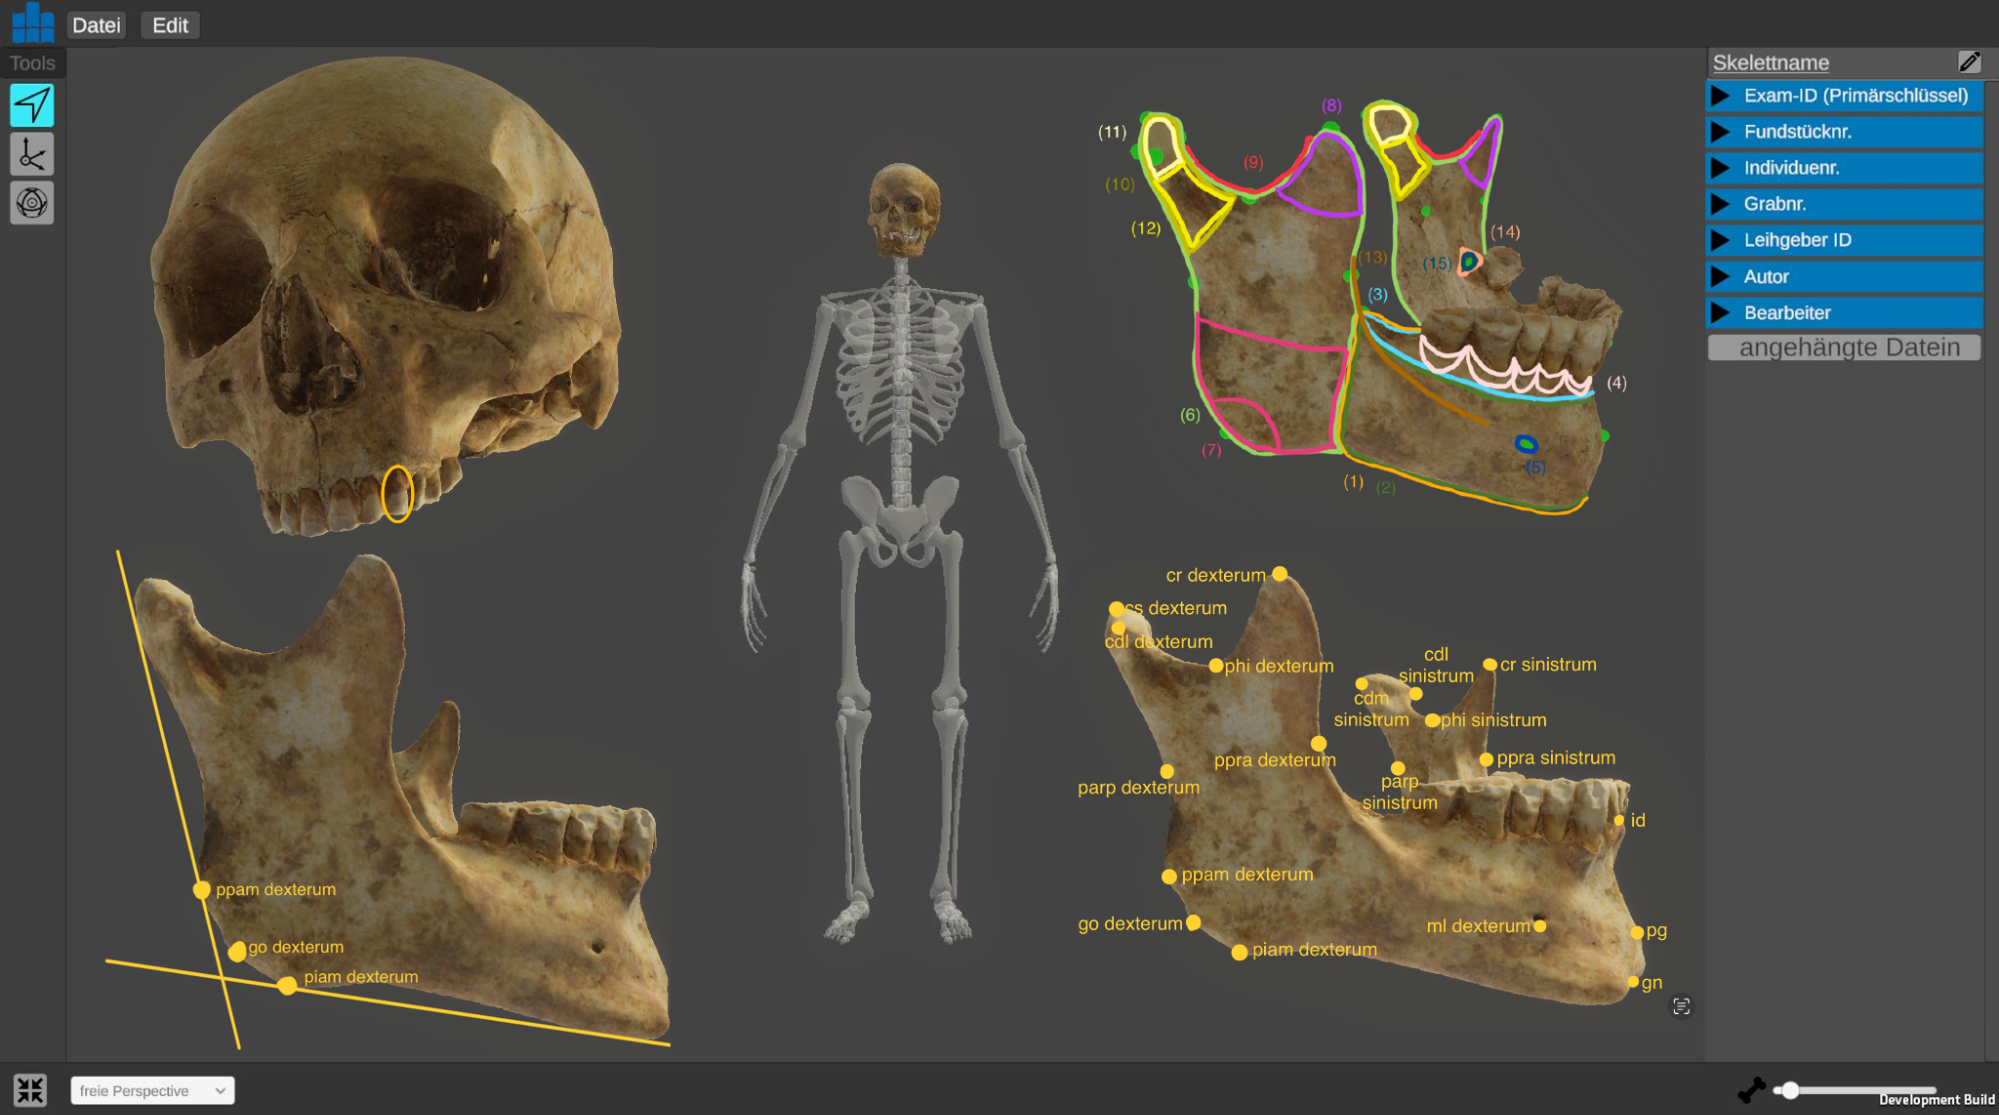
\includegraphics[width=\textwidth]{img/aw3d.png}
\caption{3D model of a Cranium (skull) inserted into a placeholder skeleton in \aw{} depicting examples of various ANNOdc classes.}\label{fig:aw3d}
\end{figure}

\begin{figure}[h]
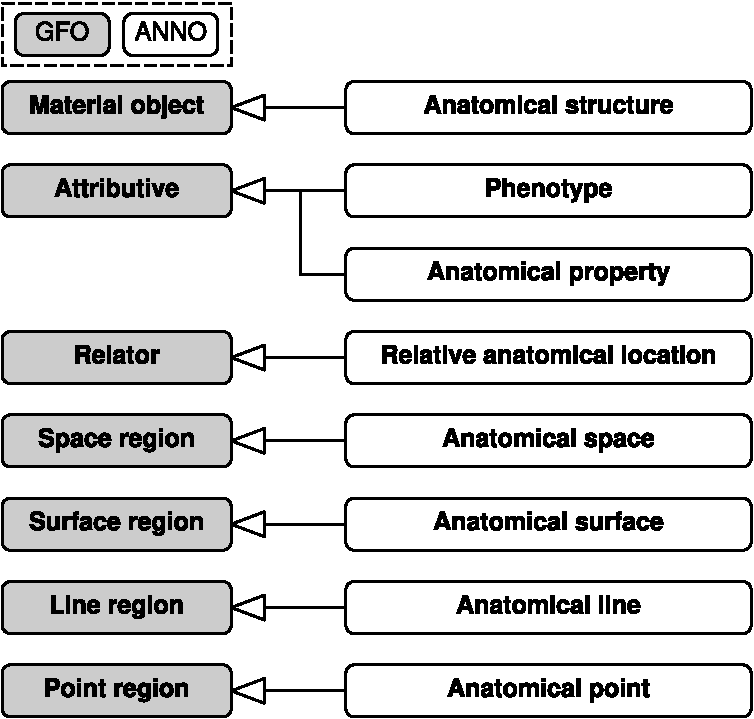
\includegraphics[width=0.6\textwidth]{img/gfo.pdf}
\caption{Integration of ANNO with the top-level GFO ontology.}\label{fig:gfo}
\end{figure}

\section{Development of ANNOds}\label{sec:domain}
% Arbeit der Domänenexperten, Tabelle, OWL-Generator
\begin{figure}[h!t]
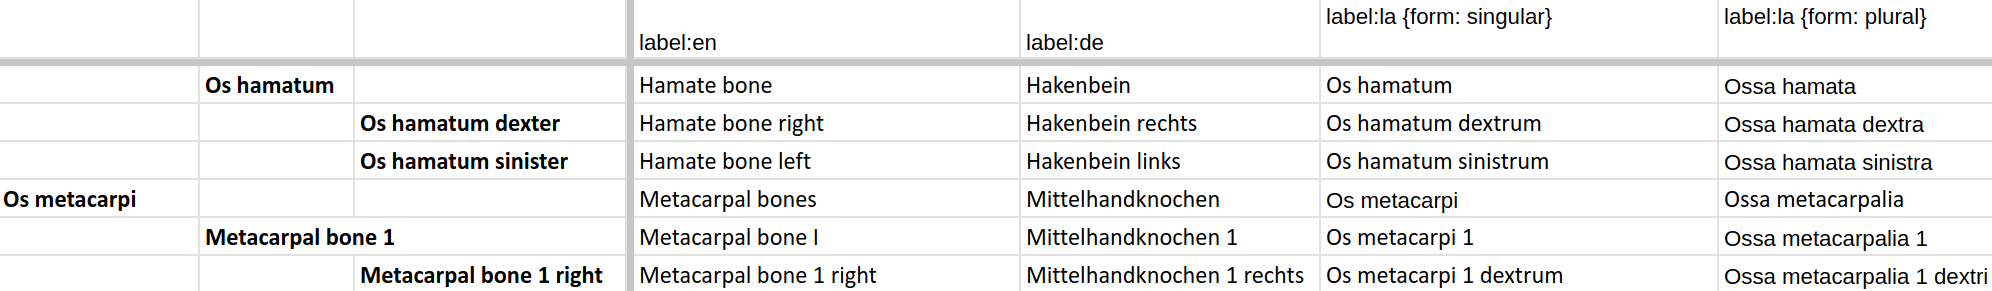
\includegraphics[width=\textwidth]{img/smog.png}
\caption{Excerpt of the spreadsheet-based input template used by the anthropologists.}\label{fig:smog}
\end{figure}

The domain experts are provided a spreadsheet-based SMOG~\citep{smog} template by the ontologists, see \cref{fig:smog}.
The spreadsheet is transformed to an OWL 2 ontology consisting of a taxonomy, annotations and some simple axioms on the basis of property restrictions.
\todo{können wir es auf OWL 2 DL eingrenzen?}

% ist das richtig übersetzt?
Sources are categorized into core, root, and occurrence sources.\todo{explain}

% Aus dem Projektbericht übersetzt
\subsection{Selection criteria}
Initially, selection criteria were made for the development of the ontology.
All bones were to be integrated.
For the individual anatomical landmarks, it was necessary to take all those that occur in the TA with the exception of anatomical variants.
However, for the cranium, the selection was reduced because the number of all ossa cranii is too high.
Overall, however, it should include those that are of anthropological relevance, i.e., contribute to navigation, localization, and identification on the bone.
Those landmarks included in the definitions of others were also to be defined.
For bones that lie on the median (e.g., mandible or sternum), bilateral landmarks were defined with side reference in each case.
For osteometric landmarks, all those already established in the core literature were to be taken.
Furthermore, those were to be taken that are relevant for meaningful measurement distances and can be annotated in \aw{}.
For measurement distances, those that are established in the bulk of the literature and core literature as well as necessary for discriminant functions and functions for body height and body weight estimation should be selected.
In addition, it also had to be integrable into \aw{}.
For the functions, those with diagnostic value were taken.
These were discriminant functions for sex determination and regression functions for body height and body weight estimation.

\subsection{Process for creating definitions and measurements}
For the definitions and measurement, a minimum amount of English-language and mostly German-language literature was compared in order to develop the definitions from their information.
Notably, Latin or ancient Greek terms were missing from the English-language literature.
The FMA also contains only English terms.
For this reason, these were also searched out with their synonyms.
Overall, the name of the landmark or survey route had to be noted in English, German, and Latin in singular and plural form, its synonyms in the three languages, the FMA and TA ID, and any information on function and delineation.
Where there were contradictions in the literature, the information was highlighted, reconciled, and logically checked.
For the osteometric landmarks, the abbreviations and their synonyms of the three languages were also provided.
Furthermore, for these as well as for the measured sections, the sources were divided into parent source, core source and occurrence source.
The parent source designates the original source of the landmark.
Under the core source, those were listed where the landmarks are listed and sampled by default.
Occurrence source represents the sources where the landmark occurs for measurements.
For redefinitions of landmarks, a meaningful Latin name had to be selected.
Requirements for this were an included position description (e.g. Punctum superioris capitis femoris as superior located point of the Caput femoris) necessary.
For this, the examination of the Latin grammar was relevant.
For the measurement sections, the type of measurement (e.g., distance measurement) and the measurement instrument were taken in addition to the name of the measurement section.
The subsequently created visual definitions were made in the different anatomical views and represented area markings for the anatomical landmarks and point markings for the osteometric ones.
\subsection{Functions}
The functions were divided into discriminant functions for sex determination and regress functions for body height and body weight estimation.
The goal here was to cover functions for at least one European, African, American, and Asian ethnicity or population.
Names were assigned by the number included in each study, the authors, and the year of publication.
In addition, the function, reference population, aspect (e.g., discriminant function), and sample size with division by gender were noted.
In addition, for the discriminant functions, the thresholds of sex assignment, classification accuracy, and misclassification were important; for the regression functions, the error interval was important.

While there are many textual sources of anthropological systematization, they do not agree in all aspects and there is not a single, formally described, standard.
ANNO links to concepts of the FMA when they exist, but structures them in a different way.

\section{Use Case: Integration into \aw{}}\label{sec:aw}
% this is based on project report but has to be rewritten: less about AW3d and more about the usage of ANNO by it
ANNO is used by \aw{}~\citep{aw3d}.
By combining user-friendly techniques of photogrammetry, insights from user experience research and knowledge from game development, a digital twin is created, which can subsequently be examined virtually.
This enables location-independent and parallel work without wear and tear on the bone.
The examination can be performed as often as desired, even if the skeletal individuals or collections are not available at the institute or have already been reburied.
It also draws its advantage when space is limited.
Thus, it requires only three SLR cameras, sufficient exposure and a computer.
The examination proceeds as follows: After photogrammetry is done and the 3D model is created, the objects are imported into the software and calibrated.
For calibration, there is an individual placeholder for each bone, which must first be selected.
Then the calibrated digital twin is placed in a placeholder skeleton.
Annotations can be made in the detailed view of each bone.
Point, line and area markings are available for selection.
Furthermore, it is possible to make measurements.
You can choose between distance, angle and circumference measurements.
After marking or measurement, an identification number is assigned to each one.
There is also a documentation about the time of the annotation as well as the name of the editor.
The marking or measurement can be classified according to certain categories (e.g. anatomical variation).
In addition, annotations are possible in a text field.
The annotations can be edited at any time afterwards, and the date of editing is recorded together with the author.
The annotations are subsequently displayed in different colors, so that overlaps can be kept apart.
A special feature of the software is the automation of measurements.
The program automatically sets pins for osteometric landmarks in a template view.
The person using the program can move these as desired.
The pins displayed have different color shades.
These differ depending on the relevance.
If the osteometric landmark is present in many measurement sections, its relevance increases and the pin appears darker.
After the pins have been roughly set, they can be refined using various views.
In the views, the individual osteometric landmarks are visible from different views, so that a fine adjustment can be made.
This is followed by the automatic measurement.
The individual values for each measurement section can be downloaded as a CSV file.
In addition, it is now possible to perform sex determinations using discriminant functions.
For this purpose, the required measurement sections can be selected.
The results are only visible in one display.
The automation allows a time saving, whereby more bones or skeletons can be examined in a shorter time.
Advantages over the previous approach are:

\begin{itemize}
\item ontology-oriented generation of placeholders/containers for objects to be imported
\item variable properties for different bone elements and bone types
\item hierarchy for orientation within an examination project according to the ontology tree
\item categorization of measurements and markers according to specifications from the ontology
\item generation of input forms based on the specified properties and bone types
\item automatic generation of measurements
\end{itemize}

%\subsection{}\label{s1.1}
~\citep{rickview}
\section{Conclusion and Future Work}
% Conclusion

% Basiert auf dem Fazit aus dem Projektbericht
ANNO introduces uniform definitions for the anatomical landmarks of the human skeletal system as well as osteometric landmarks, measurement distances and functions.
basis for anthropological work
The ontology is interlinked with ... and includes sources for all external definitions.
The ontology is used in \aw{} in place of an old, hard-coded format, which saves development time, separates annotation file compatibility from software versions, eases annotation through hierarchical browsing and increases interoperability.
% following two sentences are machine translated, improve and rewrite
It provides a basis for future training of ontologists, knowledge managers, further research activities and specialization opportunities in this field.
Furthermore, there is interest of the results in forensic, historical and prehistoric anthropology, pathology and medicine as well as in the field of computer science and especially medical informatics.
%Moreover, the ontology can be extended.

ANNO is published on \url{https://ols.imise.uni-leipzig.de} as well as \url{https://annosaxfdm.de/ontology/}.
TODO: Bereitstellung der Ontologie für die Community (OLS etc.).

% Future Work
can be extended with osteological terms of description
Arten von Erhebungen, Öffnungen, ...
anthropologische ebene draufmodellieren zb form
an anthropological landmark can have different anthropological properties

04-06 notizen
anschlussprojekte erweiterung
selbst wenn man nur einen einzelnen knöchel beschreibt wird dieser zuerst in das gesamte skelett
in der ebene zb lateral positioniert
könnte relation bestehen zwischen knochen
4 referenzpunkttypen
eine landmarke kann auf einer ebene liegen aber nicht auf einer achse, da sie keine ausdehnung hat
zb median sagital achse
Richtung vom reference point aus
location is eigenschaft der landmarke

%\begin{figure}[t]
%\includegraphics{}
%\caption{Figure caption.}\label{f1}
%\end{figure}

%\begin{table*}
%\caption{} \label{t1}
%\begin{tabular}{lll}
%\hline
%&&\\
%&&\\
%\hline
%\end{tabular}
%\end{table*}

\begin{ack}
\noindent\begin{minipage}{0.90\textwidth}
The ANNO project is co-financed from tax funds based on the budget passed by the Parliament of the Free State of Saxony.
\end{minipage}%
\hfill%
\begin{minipage}{0.04\textwidth}\raggedleft

\includegraphics[width=\textwidth]{img/saxony.pdf}
\end{minipage}
\end{ack}

\nocite{*}
\bibliographystyle{ios1}
\bibliography{paper}
\end{document}
